\section{Epipolar Geometry and Chaining}
\label{egc}
In this section we are going to describe the first step of the Structure from Motion algorithm, which is to exploit prior knowledge about the scene. This is done by finding corresponding image points in multiple views and compute their epipolar geometry which is expressed algebraically by the fundamental matrix which can be decomposed to obtain the required projection matrices.

\subsection{DataSet}
The data we were required to use consisted of two individual datasets. The first one contains 49 frames, each one of them depicting a house from a different view. The second contains 16 frames, each one of them depicting a teddy-bear from a different view. In each frame the camera movement is small, making the process of extracting structure from the scene an easier task.

\subsection{Implementation}
An important step of the algorithm is to identify local features in each image which are consistent in most of the frames. For this purpose we used a Scale-invariant feature transform (or SIFT) algorithm to detect points of interest in each frame. In order to restrict the search process of the SIFT detector an active contour based segmentation was used. By applying this technique we were able to segment the frames into background and foreground regions, allowing us to keep only the points that exist on the object of interest as can be seen in figure~\ref{fig:houseBackground}.

\begin{figure}[ht!]
  \centering
    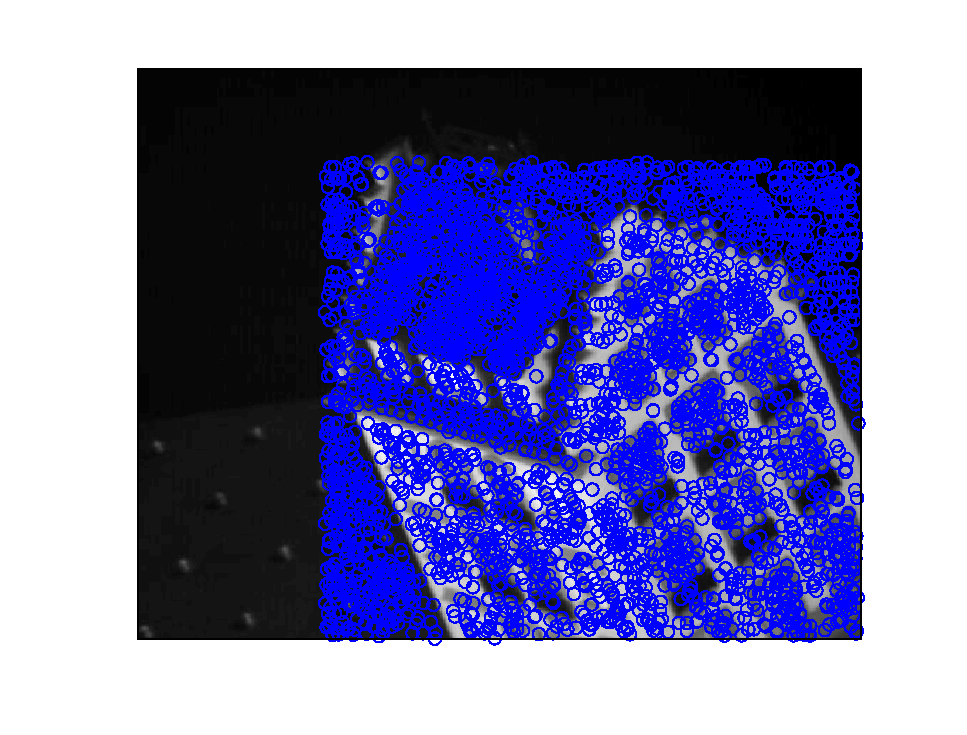
\includegraphics[width=0.55\textwidth]{figures/houseBackground.eps}
    \caption{Feature points extracted by the SIFT detector found on the object of interest}
    \label{fig:houseBackground}
\end{figure}

By finding feature points in every frame we are able to identify matches in each consecutive frame. This is done by using the build-in function VL \_ UBCMATCH of the vlFeat library of matlab which returns the qualitative corresponding feature points and rejects the ambiguous ones. Feature matches between two consecutive frames of the House dataset is displayed in figure~\ref{fig:matches}  

To estimate the fundamental matrix from the corresponding image points extracted by the SIFT detector the normalized eight-point algorithm~\cite{eight-point} was implemented. This variational algorithm leads to a more stable result than the simple eight-point implementation.  